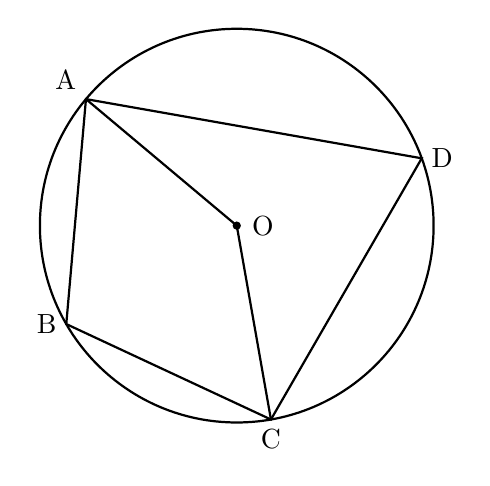
\begin{tikzpicture}[scale=1]

    % --- Coordinates ---
    % Center of the circle
    \coordinate (O) at (0,0);
    
    % Points on the circumference (approximated from the image)
    \coordinate (A) at (140:2.5);  % Top-left vertex
    \coordinate (B) at (210:2.5);  % Bottom-left vertex
    \coordinate (C) at (280:2.5);  % Bottom vertex
    \coordinate (D) at (20:2.5);   % Top-right vertex

    % --- Circle ---
    % Drawing the main circle centered at O
    \draw[thick] (O) circle (2.5);

    % --- Main Lines ---
    % Drawing the inscribed quadrilateral ABCD
    \draw[thick] (A) -- (B) -- (C) -- (D) -- cycle;
    
    % Drawing the radii OA and OC
    \draw[thick] (O) -- (A);
    \draw[thick] (O) -- (C);

    % --- Points ---
    % Marking the center point O with a dot
    \fill (O) circle (1.5pt);

    % --- Labels ---
    % Placing point labels as they appear in the original image
    \node[above left] at (A) {A};
    \node[left] at (B) {B};
    \node[below] at (C) {C};
    \node[right] at (D) {D};
    \node[right=2pt] at (O) {O};

\end{tikzpicture}